\chapter{Antecedentes} \label{cap:antecedentes}
% BREVE DESCRIPCIÓN DEL CONTENIDO DE ESTE CAPÍTULO
En este capítulo se hace una revisión de los conceptos básicos y fundamentales que serán utilizados a lo largo de este trabajo. Primero, en la sección \ref{sec:vehículos_sin_conductor}, se define el concepto de vehículo sin conductor y se responde el ¿Por qué? es necesario su desarrollo, se toman en cuenta referencias históricas en su evolución y se revisan los conceptos necesarios para que un vehículo sea considerado como autónomo. Además, se describen los niveles de autonomía que puede alcanzar un vehículo que es autónomo en base a las operaciones tácticas y operativas desempeñadas, finalmente se analiza el nivel de autonomía que puede lograr este trabajo. En la sección \ref{sec:simuladores}, se ofrece una justificación a las preguntas ¿Por qué? y ¿Para qué? usar simuladores, en las subsecciones se dar a conocer conceptos relacionados con simuladores y ejemplos de simuladores dedicados al desarrollo de robótica. Las secciones \ref{sec:conceptos_básicos_de_visión_artificial}, \ref{sec:aprendizaje_no_supervisado} y \ref{sec:máquinas_de_estados_finitos} están dedicadas a definir conceptos teóricos relacionados con el procesamiento digital de imágenes, aprendizaje no supervisado y máquinas de estados finitos respectivamente. En la sección \ref{sec:trabajo_relacionado} se abordan tecnologías y trabajos relacionados con este proyecto.

\section{Vehículos sin conductor} \label{sec:vehículos_sin_conductor}

Vehículo autónomo, automóvil sin conductor, automóvil con conducción automática o vehículo guiado automatizado son algunos de los nombres que hacen referencia al concepto de conducción autónoma. De manera general, un vehículo autónomo se define como cualquier vehículo de pasajeros que es capaz de conducirse por si mismo. Sin embargo, se requiere de un mecanismo de control bien estructurado para llevar a cabo la tarea de conducción autónoma \cite{rathod2013autonomous}.

Existen registros acerca de la historia de los automóviles autónomos donde se indica un comienzo en los Estados Unidos en la primera mitad del siglo XX, al rededor de los años 1920 debido al constante y fuerte aumento de accidentes de tránsito,se estimaron al menos 200 mil muertes accidentales provocadas por transportes motorizados en aquella época, donde el mayor número de estas defunciones fueron peatones y no conductores. El error humano fue concebido como la principal causa de dichos accidentes. Sin embargo, el diseño e infraestructura de los autos de la época también fueron factores críticos que influyeron directamente en la forma y gravedad de los percances viales, fue entonces que surgió la idea de sustituir a humanos propensos a errores con tecnología que permitiera un mejor desempeño.

De esta manera inició el desarrollo de nuevas tecnologías que permitieran un acercamiento a la conducción autónoma. Algunos desarrollos previos tomaron mayor fuerza. Lawrence B. Sperry usó el primer giroscopio estabilizador de avión en junio de 1914, este es considerado hasta la actualidad como el primer piloto automático. Otro de los adelantos tecnológicos de la época fueron las ondas de radio, esta nueva ciencia de radio-guía se vio comprometida con el control remoto de mecanismos en movimiento a través de ondas de radio. Esta tecnología fue desarrollada, entre otros, por el ejercito de los estados unidos, con el objetivo de controlar misiles, barcos y aviones a distancia. Para el año de 1921 estos trabajos pioneros vieron como resultado el primer vehículo sin conductor. Ingenieros del \textit{Radio Air Service} presentaron al público un automóvil de 2.5 metros de largo  que fue controlado por medio de ondas de radio desde un camión del ejército que conducía 30 metros por detrás del vehículo. En el estricto sentido no se trataba de un vehículo con conducción autónoma, sino de uno controlado a distancia con el conductor fuera del auto. Una situación que resulta digna de mención es que la historia y los fundamentos de los autos sin conductor esta fuertemente relacionada con el ejército y los avances impulsados por conflictos bélicos.

En la actualidad y de acuerdo con datos de la OMS en promedio suceden 1.24 millones de defunciones en el mundo relacionadas con accidente viales por año\cite{lenz2016autonomous}. Una gran parte de estos accidentes son ocasionados por fallos humanos debido a que la cantidad de asistencia que requiere un conductor o usuario es muy demandante, pues se enfrenta a actividades exhaustivas como tráfico intermitente, tramos largos en carreteras, estar bajo influencia de medicamentos o algún otro agente y cansancio excesivo, son algunos factores que al final terminan con cualquier placer de conducir. En cualquiera de estos casos, la capacidad de un vehículo autónomo abre nuevas oportunidades a una mejor movilidad y optimización en el flujo de tráfico.

\subsection{Aspectos necesarios para un vehículo autónomo} \label{sub:aspectos_necesarios_para_un_vehículo_autónomo}

Uno de los principales retos de los vehículos autónomos es disminuir el número de accidentes vehiculares, pues ya se han mencionado pruebas evidentes para afirmar que la mayoría de los accidentes automovilísticos son ocasionados con mayor frecuencia por errores humanos. Además, prometen numerosas mejoras para el tráfico vehicular, aumento en la capacidad de las carreteras y mejoras en el flujo de tráfico debido a tiempos de respuesta más rápidos, también se estima menor uso de combustible y disminución de emisiones contaminantes como consecuencia de una conducción más previsora pero sobre todo supervisada por agentes inteligentes.\cite{luettel2012autonomous}

Una plataforma robusta de un vehículo autónomo es esencial para lograr la operación del mismo en condiciones reales y ambientes urbanos. Principalmente esta plataforma está compuesta de:
\begin{enumerate}
    \item \textbf{Hardware}: Representado por toda la arquitectura física para reconocer el ambiente y actuadores capaces de interpretar información de los sensores, la figura \ref{fig:self_driving_car} ilustra esto. Un hardware dedicado a vehículos autónomos consta de tres bloques esenciales.
    % \footnote{\url{https://softwareengineeringdaily.com/}} 
    \begin{itemize}
        \item Sensores: Para percibir el entorno y sus movimientos, es común el uso de cámaras estéreo, RGB y RGB-D, dispositivos para realizar mediciones de rango como sensores RADAR y LIDAR, GPS para información de odometría.

        %Con el fin de estimar el movimiento del vehículo se emplean mediciones de odometría e inercia, estas mediciones son principalmente otorgadas por sensores GPS.

        %En el caso de las tecnologías láser como el sensor LIDAR es indispensable realizar una tarea de calibración previa al uso. Para el LIDAR es común usar calibración extrínseca e intrínseca con el fin de mejorar el desempeño del sensor y obtener lecturas más confiables.
        \item Actuadores: Permiten realizar acciones de control en el vehículo
        \item Ordenadores: Para procesar entradas y generar salidas.
    \end{itemize}
    
    \item \textbf{Software}: Son todos aquellos módulos lógicos que hacen uso de la información de sensores, se encargan de procesarla mediante algoritmos específicos \cite{levinson2011towards}. Entre las principales tareas que realiza el software de un vehículo autónomo destacan.
    \begin{itemize}
        \item Mapeo del ambiente
        \item Localización
        \item Planificación de rutas
        \item Reconocimiento y percepción del ambiente
        \item Modelado de leyes de control
    \end{itemize}
\end{enumerate}

\begin{figure}
    \centering
    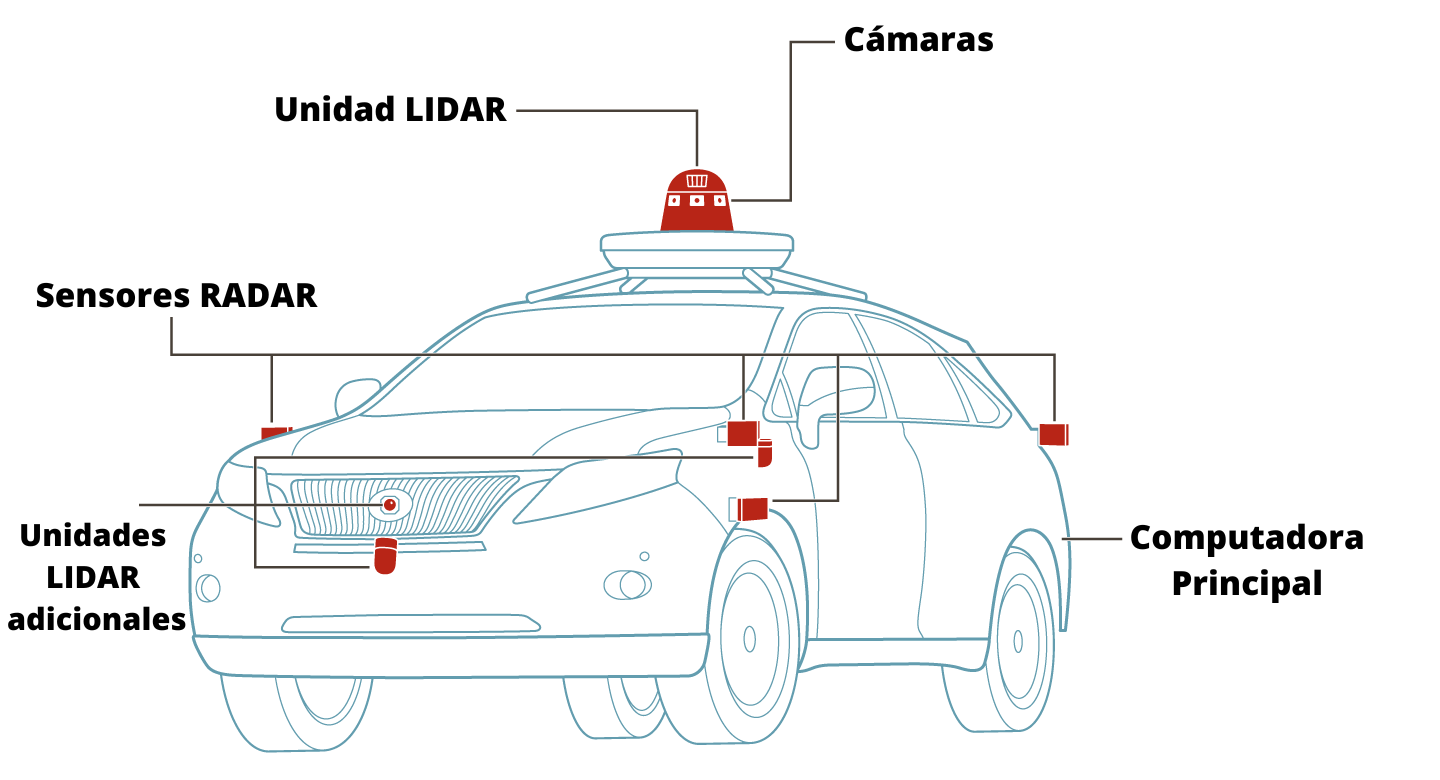
\includegraphics[width=0.7\textwidth]{Figures/Figures_Cap02/self_driving_car.png}
    \caption{Hardware dedicado a vehículos autónomos.}
    \textit{Nota}. Adaptada de \textit{Software Engineering Daily}, 2018 \cite{SoftwareEngineeringDaily}.
    \label{fig:self_driving_car}
\end{figure}

\subsection{Niveles de autonomía} \label{sub:niveles_de_autonomía}

Conducir un vehículo requiere ejecutar gran variedad de acciones y toma de decisiones ya sea si el vehículo se encuentra en movimiento constante o bien, estático en una situación de tráfico. El acto de conducir se puede clasificar en tres diferentes tipos de esfuerzo que realiza el conductor: estratégico, táctico y operativo\cite{michon1985critical}. Los niveles de autonomía de un vehículo motorizado sin conductor se refieren al nivel de ayuda que provee el sistema de automatización con el que está instrumentado. Es decir, el nivel de autonomía es otorgado según el grado de asistencia que se ofrece en la tarea de conducción dinámica.

El término Tarea de Conducción Dinámica o DDT (\textit{Dynamic Driving Task}) por sus siglas en inglés es el concepto que se atribuye a la suma de esfuerzos o funciones tácticas y operativas ejecutadas en tiempo real necesarias para un vehículo en carretera. Otras subtareas como la selección de destinos, programación de viajes y puntos de referencia están excluidas del concepto de DDT porque pertenecen al grupo de funciones estratégicas. Los esfuerzos operativos y tácticos son complementarios, en conjunto resultan como la acción de operar un vehículo\cite{sae2021surface}. De acuerdo con la clasificación de Michon en 1985, el esfuerzo estratégico implica la planificación del viaje, decidir cuándo y dónde ir, cómo viajar, además de elegir la mejor ruta. El esfuerzo táctico incluye técnicas de maniobra durante el trayecto del viaje, esto incluye la toma de decisiones de cómo y cuándo se puede rebasar a otro vehículo, cambiar de carril, mantener velocidad adecuada, revisión de retrovisores laterales y superiores. La última categoría es el esfuerzo operativo que hace referencia a aquellas acciones consideradas innatas o constantes, como es realizar pequeñas correcciones del ángulo de dirección con el volante para mantener el vehículo estable, frenar y acelerar para evitar obstáculos repentinos o eventos peligrosos en el camino\cite{michon1985critical}. 

Ejemplos de funciones operativas y tácticas son:
\begin{enumerate}
\item Operativas
    \begin{itemize}
        \item Control de movimiento lateral por medio de la dirección (\textit{Steering}).
        \item Control de movimiento longitudinal a través de aceleración y desaceleración.
    \end{itemize}
\item Tácticas
    \begin{itemize}
        \item Planificación de maniobras.
        \item Evasión de obstáculos y seguimiento de rutas.
    \end{itemize}
\item Operativas y Tácticas
    \begin{itemize}
        \item Supervisión del ambiente de conducción: detección,  reconocimiento y  clasificación de objetos.
        \item Ejecución de respuesta ante eventos y objetos (OEDR).
    \end{itemize}
\end{enumerate}

La Sociedad de Ingenieros Automotrices (SAE) ha desarrollado un estándar que define la escala de niveles de autonomía. Esta escala determina 6 niveles de autonomía para conducción automática,  desde el nivel 0 (Sin Conducción Automática) hasta el nivel 5 (Conducción Automática Completa)\cite{sae2021surface}. En breve, se enuncian y describen los 6 niveles propuestos por la Sociedad de Ingenieros Automotrices (SAE).

\begin{itemize}
    \item \textbf{Nivel 0: \textit{No Driving Automation}} 
    
    El nivel 0 implica que el conductor es completamente responsable del control de vehículo, es decir, se encarga de las funciones tácticas y operativas. Aunque los vehículos de nivel 0 cuenten con características de seguridad que ayuden a los conductores como: advertencias de colisión y punto ciego, frenado automático de emergencia e incluso cámaras de retroceso,  se clasifican dentro del nivel 0 porque ninguna de estas características actúan durante un periodo prolongado.
    
    \item \textbf{Nivel 1: \textit{Driver Assistance}} 
    
    En el nivel 1 el sistema de conducción automatizado (ADS) toma control del vehículo en situaciones muy específicas. Tal es el caso de control de movimiento lateral y longitudinal, pero no ambas simultáneamente. Esto quiere decir que se mantiene la expectativa de que el conductor realice el resto de la DDT. Un ejemplo es el sistema ACC (\textit{Adaptative Cruise Speed}) que controla la aceleración y el frenado, generalmente en conducciones largas sobre carretera.
    
    \item \textbf{Nivel 2: \textit{Partial Driving Automation}} 
    
    Este nivel de autonomía presenta mejoras en el reconocimiento del entorno y permite al vehículo realizar acciones más complejas. En el caso de control longitudinal para aceleración y frenado, para control lateral ayuda en la corrección de dirección.
    
    De manera general, el nivel 2 provee ayuda por parte del sistema de conducción automatizado (ADS) para cumplir un porcentaje de la tarea de ejecución de respuesta ante eventos y objetos para completar acciones de control en movimiento lateral y longitudinal con asistencia limitada. Existen eventos ante los cuales el sistema no es capaz de responder y por lo tanto, el conductor debe de supervisar el desempeño de la asistencia proporcionada con el  propósito de completar la conducción dinámica (DDT).
    
    \item \textbf{Nivel 3: \textit{Conditional Driving Automation}} 
    
    El nivel 3 es considerado el punto de entrada a la conducción autónoma, pues en situaciones muy específicas con cierto tipo de carreteras y condiciones climáticas adecuadas el conductor comienza a desconectarse del acto de conducir.  
    
    El desempeño por parte del sistema de conducción automatizado es considerablemente mejor, pues toma el control de todas las acciones que permiten completar la tarea de conducción dinámica (DDT). En este nivel aún se mantiene la expectativa de que el conductor este listo ante las solicitudes que pueda requerir el ADS para retomar el control del vehículo en cualquier momento. Un ADS de este nivel permite completar un conducción dinámica en condiciones específicas, por ejemplo en autopistas con velocidad moderada y manejo de frenos. En situaciones de tráfico intermitente el vehículo envía alertas al conductor para que retome el control.
    
    \item \textbf{Nivel 4: \textit{High Driving Automation}} 
    
    En este nivel el sistema de conducción automatizado es completamente capaz de vigilar el entorno de conducción y ejecutar funciones tácticas y operativas. El vehículo también cuenta con la capacidad de alertar al conductor si es que los límites operativos se sobrepasan, en caso de no encontrar respuesta por parte del conductor el vehículo debe asegurarse automáticamente. En otras palabras, un usuario dentro de un vehículo adaptado con características de nivel 4 es un pasajero que no necesita responder ante fallas del sistema.
    
    El cumplimiento de condiciones de riesgo mínimo en adición con la capacidad de recuperación automática resultan ser la principal diferencia que ofrece el ADS  de nivel 4 frente a uno de nivel 3. Vehículos adaptados con condiciones de nivel 4 son capaces de seguir una ruta predeterminada dentro de regiones geográficas limitadas; por ejemplo: circuitos cerrados, campus escolar o una base militar.
    
    %Un ADS diseñado para el nivel 4 está capacitado para cumplir conducción dinámica hacia adelante y hacia atrás, además de lograr una conducción con riesgo mínimo en caso de que el usuario no pueda retomar el control. 
    
    \item \textbf{Nivel 5: \textit{Full Driving Automation}} 
    
    Los vehículos adaptados a un nivel 5 de autonomía son completamente independientes, es decir, el usuario no necesita supervisar el sistema de conducción automatizado. Esto significa que el ADS puede controlar el vehículo dentro de cualquier carretera en cualquier lugar del mundo bajo las mismas condiciones en las que un humano lo pueda hacer.
    
    Esto quiere decir que no existen restricciones climáticas, geográficas o de horario donde pueda operar. Sin embargo, esto no significa que un vehículo del nivel 5 pueda actuar en situaciones donde resulte imposible la tarea de conducción dinámica incluso para los humanos; por ejemplo en tormentas de nieve, derrumbes o inundaciones. En tales casos el ADS debe de lograr una condición de riesgo mínimo, deteniéndose o esperando a que las condiciones cambien. Un vehículo en este nivel puede ser programado con un punto de inicio y un punto de destino siendo capaz de cubrir el trayecto completo en vías públicas independientemente de las condiciones de tráfico, carretera y o clima.
\end{itemize}


%De manera mas concisa se pueden expresar las acciones de manejo que ejecuta el conductor y el sistema de conducción automatizado según el nivel en el que se encuentre.

A partir del nivel 0 y hasta el nivel 3 se entiende que el conductor tiene mayor grado de responsabilidad sobre el manejo del vehículo. El conductor debe de supervisar constantemente las funciones de apoyo con las que cuente el vehículo, según el nivel. Sin embargo, debe de mantenerse atento para frenar, acelerar y dirigir según sea necesario. Un sistema de conducción automatizado (ADS) de estos niveles cuenta con características que permiten proporcionar asistencia y advertencias momentáneas en el caso del nivel 0 por medio de frenado de emergencia automático (AEB)  y advertencia de punto ciego. En los niveles 2 y 3 existen características que ayudan en acciones de control lateral y longitudinal del vehículo como: sistemas ACC y centrado de carril \cite{sae2021surface}.

Los niveles 3, 4 y 5 brindan un mayor grado de asistencia y en consecuencia producen una disminución en las tareas que debe desempeñar el conductor. Para el caso de los niveles 3 y 4 la conducción autónoma es limitada y restringida, el usuario solo retoma el control del vehículo si el sistema de conducción lo solicita. El nivel 5 de autonomía permite navegación de manera completa en cualquier lugar y sin restricciones, el ADS de este sistema esta conformado por una combinación y mejora de cada uno de los componentes usados en niveles inferiores\cite{sae2021surface}.

%en el nivel 5 no se requiere que el conductor se haga cargo de la unidad. 

%La conducción autónoma es limitada y restringida en los niveles 3 y 4, esto se logra por medio de una mayor percepción del ambiente de conducción, en estos dos casos no es necesaria la presencia del conductor al frente del volante, solo si es solicitado por el ADS. 

\subsection{Nivel de autonomía esperado en este trabajo} \label{sub:nivel_de_autonomía_esperado_en_este_trabajo}

En este trabajo se pretende alcanzar un nivel 4 de autonomía, con el fin de lograr este nivel se planea instrumentar un vehículo(simulado en 3D) con sensores que le permitan percibir el ambiente de conducción. LIDAR, cámaras RGB y GPS ayudarán en la estimación de objetos para resolver acciones de rebase y seguimiento de carriles.

También se buscan desarrollar las leyes de control correspondientes para el desempeño de tareas operativas y tácticas de conducción dinámica (DDT). Es considerado como nivel 4 por las características que posee el sistema de conducción automatizada (ADS), además de que la intervención humana es casi nula, pues al ser un ambiente simulado no se cuentan con estas características. Funciones estratégicas quedan fuera del alcance de este trabajo.

\subsection{Sensores} \label{sub:sensores}

\begin{itemize}
    \item \textbf{LIDAR}: \textit{Light Detection and Ranging} por sus siglas en inglés es una tecnología óptica utilizada para detección de objetos, es decir, permite medir distancia y otras propiedades de un objeto objetivo que es iluminado por un haz de luz, a menudo se hace por medio de pulsos láser. Luz ultravioleta, visible o infrarroja son ejemplos de luz que puede usar un sensor LIDAR. Objetos no metálicos, rocas, compuestos químicos, sólidos, nubes e incluso moléculas individuales son ejemplos de objetos que puede detectar este sensor \cite{rathod2013autonomous}.
    % El LIDAR esta diseñado para medir información de rango y proporcionarla al usuario. 
    El principio fundamental de el funcionamiento del LIDAR es emitir un pulso de luz hacia el objetivo y por consecuencia activar un circuito interno de temporización. Internamente se calcula el tiempo que le toma al láser llegar al objetivo y regresar al receptor desde el objetivo, este proceso obtiene la distancia a la que se encuentra el objeto objetivo. Sin embargo, la información que se presenta al usuario puede no estar en un rango real debido a diferentes factores externos, por ejemplo; el ruido inherente del ambiente.

    %puede provocar variaciones inesperadas en sensores de baja escala de hasta 10 centímetros en mediciones de rango, estas variaciones resultan ser perjudiciales en aplicaciones de navegación autónoma o en aplicaciones donde se requiera de una precisión con mayor exactitud\cite{cooper2018range}.
    
    \item \textbf{Cámaras RGB}: Uno de los sensores más complejos utilizados en la robótica son las cámaras digitales. Las cámaras digitales son capaces de capturar y almacenar imágenes digitalmente. De este modo, una cámara RGB es capaz de medir la capacidad de luz dentro de un espectro visible, es decir, el mismo espectro que pueden ver los ojos humanos. Mediante un cámara RGB se pueden captar e interpretar la gama de colores que percibimos los humanos. A diferencia de las cámaras en escala de grises, una cámara RGB agrega una capa de pintura sobre la máscara de píxeles, entonces cada píxel solo registra la intensidad de una determinada componente de color \cite{braunl2003embedded}.
    
    \item \textbf{Cámaras Estéreo}: Una cámara estéreo es un tipo de cámara digital que intenta simular la visión humana y cuenta con la capacidad de capturar imágenes tridimensionales. Una cámara estéreo posee dos o más lentes con un sensor de imagen separado para cada lente, la distancia entre lentes es aproximadamente la distancia promedio en los ojos humanos. Su funcionamiento se basa en tomar una imagen por cada sensor en el mismo instante, luego mezclarlas y obtener como resultado un imagen 3D. El uso de cámaras estéreo es amplio en el sector tecnológico con diferentes campos de aplicación como: vehículos autónomos, astronomía, medicina, topografía, entre otros.
    
    \item \textbf{Cámaras RGB-D}: Las cámaras digitales convencionales producen imágenes como una matriz bidimensional. Por lo general, cada píxel tiene valores asociados al rojo, verde y azul, o RGB. Cada atributo va desde 0 hasta 255, por lo que el color negro es una combinación $(0, 0, 0)$ y un rojo brillante puro sería $(255, 0, 0)$. Juntos miles o millones de píxeles crean este tipo de imágenes. Por otro lado, una cámara de profundidad, tiene píxeles con un valor numérico diferente asociado a ellos, este número representa la distancia o profundidad desde la cámara. 
    Existe diferentes métodos para calcular la profundidad, este se elige según la aplicación en turno. Algunas cámaras de profundidad combinan sistemas RGB más un sistema de profundidad y por lo tanto generan píxeles con los cuatro valores mencionados, o RGBD \cite{cameraRGBD}.
    % \footnote{\url{https://www.intelrealsense.com/beginners-guide-to-depth/}}
    
    \item \textbf{Sonares}: El propósito de los sensores sonares es emitir una señal acústica corta con una frecuencia ultrasónica en un rango de $[50, 250]$ kHz, luego, calcula el tiempo desde la emisión hasta que el eco vuelve al sensor. Este tiempo es proporcional al doble de la distancia del objeto más cercano. Si no se recibe ninguna señal de vuelta en un lapso de tiempo, entonces ningún objeto es detectado en la distancia correspondiente \cite{braunl2003embedded}. 
    Durante décadas, los robots móviles han sido instrumentados con diferentes sensores para navegación, debido a esto, los sensores para medir distancias se encuentran entre los más importantes en robótica. A pesar de lo poderoso que son los sonares en detección de objetos, también poseen desventajas, por ejemplo; interferencias y reflejos. La interferencia ocurre cuando se operan varios sensores de sonar a la vez, por otro lado, los reflejos pueden implicar que un obstáculo parezca estar más lejos de lo que en realidad está.
    
    \item \textbf{GPS}: El sistema de posicionamiento global o GPS de sus siglas en inglés es un sistema de navegación que usa satélites, un receptor y algoritmos para sincronizar información de ubicación, velocidad y tiempo. Se compone de tres componentes diferentes, conocidos como segmentos (satélites, control terrestre, equipo de usuario) y trabajan conjuntamente para proporcionar información de ubicación. El conjunto de satélites utilizado por los GPS consta de una constelación con 24 satélites repartidos en 6 planos orbitales alrededor del planeta Tierra. Solo son requeridos tres satélites para producir una ubicación en la superficie terrestre, sin embargo, a menudo se usa un cuarto satélite para validar información de los otros tres. Además, el cuarto satélite permite calcular la altitud de un dispositivo \cite{gps}.
    % \footnote{\url{https://www.geotab.com/blog/what-is-gps/}}

    Actualmente el uso de GPS está presente en la industria de localización, navegación, seguimiento de objetos, creación de mapas del mundo, entretenimiento, vehículos autónomos, seguridad y comunicaciones móviles.

    %Estos tres segmentos son: \textbf{Satélites}: Giran al rededor de la Tierra y transmiten señales de posición y tiempo, \textbf{Control terrestre}: Son estaciones de monitoreo terrestre, estaciones de control y antenas terrestres para seguimiento y control de satélites en el espacio, \textbf{Equipo de usuario}: Son receptores y transmisores GPS como teléfonos inteligentes, dispositivos telemáticos, entre otros.
\end{itemize}

%\textcolor{red}{Comienza por hablar sobre qué es un vehículo sin conductor y qué características tiene. Tal vez menciona un poco de la historia. Sobre definiciones, puedes encontrar información en:  \url{https://core.ac.uk/download/pdf/234677061.pdf} \url{https://link.springer.com/book/10.1007/978-3-662-48847-8}}

%\textcolor{red}{Habla también sobre los niveles de autonomía y da una breve descripción de cada nivel. Enfatiza el nivel que se logrará en este trabajo. \url{https://www.sae.org/standards/content/j3016_202104/} \url{https://ieeexplore.ieee.org/document/7490340}  \url{https://www.sciencedirect.com/science/article/pii/S095741742030628X?casa_token=WTcFlQ-e2BcAAAAA:KSyYhNe1sPvDkBOi1M2HOrrKU_eX9tIiiLX4AAyAJzDQ8ECByLqFc9RDGbMLDwqU99FljAqykWE}}

%\textcolor{red}{Luego habla de lo que se necesita para que un vehículo pueda ser autónomo: \url{http://ieeexplore.ieee.org/document/6179503/} \url{https://ieeexplore.ieee.org/abstract/document/5940562}}

%\textcolor{red}{Luego hablas de los sensores más comunes que se pueden usar para instrumentar un vehículo sin conductor. Aquí hay una posible lista: \url{https://ieeexplore.ieee.org/stamp/stamp.jsp?arnumber=6179503}}
%\textcolor{red}{
%\begin{itemize}
%    \item Lidar: Cap 8 de \url{https://www.taylorfrancis.com/books/mono/10.1201/b22159/introduction-laser-science-engineering-travis-taylor}
%    \item Cámaras RGB: Cap 1 de \url{https://www.pearson.com/us/higher-education/program/Forsyth-Computer-Vision-A-Modern-Approach-2nd-Edition/PGM111082.html}  Sec. 3.9 de \url{https://www.springer.com/gp/book/9783540343196}
%    \item Cámaras estéreo: Cap 1 de \url{https://www.wiley.com/en-us/An+Introduction+to+3D+Computer+Vision+Techniques+and+Algorithms-p-9781119964476}
%    \item Cámaras RGB-D: \url{https://ieeexplore.ieee.org/document/6619001}
%    \item Sonares Sec. 3.6 de \url{https://www.springer.com/gp/book/9783540343196}
%\end{itemize}
%}

\section{Simuladores} \label{sec:simuladores}

El desarrollo de nuevas tecnologías y agentes inteligentes se encuentra en constante crecimiento a nivel mundial y los vehículos autónomos no son la excepción, debido a la creencia de que los vehículos autónomos pueden ayudar e incluso mejorar tareas de conducción dinámica, comodidad y calidad en viajes. Sistemas inteligentes como ACC, LKA, CA, DN ofrecen mayor eficiencia y confianza en condiciones normales de manejo, en situaciones de tráfico mejoran el rendimiento de combustible y mantienen un ambiente seguro.

El creciente interés en el área de  vehículos inteligentes requiere la innovación de más y mejores componentes que instrumenten a un vehículo que pretende ser autónomo. Una gran variedad de sensores, redes de sensores, tecnologías de comunicación, poder de cómputo y controladores requieren de constantes mejoras y actualizaciones en hardware y software\cite{eskandarian2012handbook}.  En este caso los simuladores son un gran aliado en el diseño y testeo de estos componentes.

%Además, el uso de tecnologías de comunicación abre puertas hacia la generación de nuevos productos y servicios que se basan en la comunicación entre vehículos en un sistema de carretera.

\subsection{¿Por qué usar simuladores?} \label{sub:por_qué_usar_ simuladores}

El desarrollo sistemas para agentes inteligentes en vehículos autónomos es un proceso complejo que involucra diferentes componentes tecnológicos, en específico electrónicos y mecánicos que en conjunto resultan ser difíciles y costosos de conseguir en caso de no contar con los recursos necesarios. Esta es la principal razón para considerar el uso de simuladores durante el desarrollo de sistemas dedicados a vehículos autónomos. Los simuladores permiten realizar desarrollos de muy bajo costo en escenarios similares al mundo real. Otra razón de mucho peso es la seguridad y robustez ante fallos, pues al usar un ambiente simulado se tiene mayor margen de maniobra ante situaciones catastróficas que en un ambiente real podrían resultar perjudiciales.

La simulación juega un papel fundamental en la evaluación y validación del desarrollo de sistemas inteligentes. Además, visto desde otro punto de vista los simuladores poseen características que permiten observación de diferentes conductas en situaciones viales para la formulación de nuevas políticas que permitan mejorar la movilidad. Convirtiéndose entonces en una herramienta para investigar escenarios futuros\cite{eskandarian2012handbook}.

\subsection{¿Para qué usar simuladores?} \label{sub:para_qué_usar_simuladores}

Como se mencionó anteriormente, cumplir con las condiciones y elementos necesarios para el desarrollo de sistemas inteligentes en vehículos autónomos está lleno de riesgos, es a largo plazo, costoso y complejo. Es por ello que el uso de simuladores se vuelve esencial en este desarrollo. 

Los simuladores en este caso ayudan a identificar diferentes aspectos para:
\begin{itemize}
    \item Conceptualizar la idea principal con base de nociones teóricos y modelos matemáticos.
    \item Implementar de ideas con tecnologías que permitan describir el comportamiento esperado.
    \item Desarrollar sistemas completos y creación de prototipos.
    \item Desarrollar productos finales con base en prototipos, sin dejar de lado el mantenimiento y actualizaciones.
\end{itemize}

%De esta manera durante la etapa de desarrollo se buscan cubrir diferentes fases con el fin de lograr la tarea final, como en cualquier proyecto de software se busca minimizar un problema de gran escala en problemas más pequeños y específicos.  
En el caso específico de vehículos sin conductor se buscan simulaciones que permitan diseñar entornos semejantes a condiciones de conducción vehicular en el mundo real. Estos simuladores distinguen diferentes tipos de simulación:
\begin{itemize}
    \item \textbf{Simulación de Tráfico:} Pretende una simulación de todos los sistemas relacionados con el tráfico (control y gestión de tráfico), su propósito es estudiar a los actores involucrados en una red de tráfico (vehículos, conductores, sistemas de tráfico) además de impactos directos en la eficiencia y seguridad del tráfico.
    
    \item \textbf{Simulación de aplicaciones y vehículos:} Es una simulación con mayor detalle de tráfico e involucra más unidades vehiculares en una red de tráfico. El objetivo de esta simulación es el desarrollo de aplicaciones y evaluación técnica.
    %los cuales son modelados con alta fidelidad, se incluyen simulaciones de hardware y software en bucle (HiL, SiL).
    
    \item \textbf{Simulación de comunicación:} El desarrollo de aplicaciones y evaluación del rendimiento de comunicación entre aplicaciones es el propósito de esta simulación. La simulación de comunicación se puede presentar en diferentes niveles según las necesidades y capacidad de computo disponibles.
    %La necesidad de simular telecomunicaciones surgió con la llegada de sistemas cooperativos,
    
    \item \textbf{Simulación de conducción:} Quizás la más importante de las simulaciones es la representación de un conductor, algunas de las funciones no son completamente inteligentes sino que resulta en una cooperación entre conductor y sistema. El objetivo de esta simulación es evaluar el comportamiento de un conductor y el efecto que tiene sobre alguna función específica.
\end{itemize}

Cada ambiente de simulación tiene sus propias necesidades para modelar y describir la dinámica de los actores presentes. Para simular funciones inteligentes en vehículos se requiere de modelos que describan la dinámica del vehículo, sensores, actuadores, conductores, rendimiento de comunicaciones y unidades de carretera. Según las necesidades, en algunos casos los modelos pueden ser reemplazados por simuladores dedicados, como el caso de telecomunicaciones a gran escala donde son manejadas por medio de  modelos estadísticos\cite{eskandarian2012handbook}.

Claramente se puede afirmar que la coherencia entre cada una de las fases de desarrollo de sistemas inteligentes en vehículos es vital con el fin de salvaguardar la portabilidad de resultados. De esta manera se obtiene un marco de trabajo que permite una simulación con diferentes niveles de detalle desde modelos de controladores hasta modelos detallados de sensores y actuadores que al final resultan en procedimientos avanzados de prueba en cada paso de simulación.

\subsection{Motores de físicas, ODE y otros} \label{sub:motores_de_físicas_ODE_y_otros}

Un motor de físicas es un software con la capacidad de realizar simulaciones de comportamientos físicos como: cinemática, dinámica de cuerpos rígidos y blandos, elasticidad, movimiento de fluidos, colisiones. Realizan las operaciones correspondientes para estos comportamientos físicos. Además, manejan los comportamientos de manera independiente del entorno, es decir, reusan código para diferentes situaciones por medio de parámetros. Existe un clasificación para los motores de físicas de acuerdo con la capacidad de procesamiento que requieran: simulación en tiempo real y los de simulación de alta precisión. Las simulaciones de alta precisión requieren de mucha capacidad de computo y generalmente son utilizados con fines científicos, por otro lado las simulaciones en tiempo real se centran más en el campo de los videojuegos.

\textbf{ODE} (\textit{Open Dynamics Engine}) es una biblioteca de gráficos profesional desarrollada en C y C++ y de alto rendimiento para simular dinámicas de cuerpos rígidos. Posee funciones estables, maduras, fáciles de usar y también añade detección de colisiones con fricción. ODE es útil en simulaciones de vehículos, objetos en entornos de realidad virtual y criaturas virtuales. Este motor prioriza la velocidad y estabilidad dejando de lado la precisión física, esto lo hace robusto y confiable pero también poco preciso respecto a otros motores en el mercado. Sin embargo, cuenta con la capacidad de personalizar el entorno incluso durante la simulación \cite{ode}.
% \footnote{\url{https://www.ode.org/}}

Actualmente es utilizado en la industria de videojuegos de ordenador, creación de modelos 3D y herramientas de simulación. Otros motores de físicas importantes para simulaciones en tiempo real y de alta precisión son:
\begin{itemize}
    \item \textbf{Tiempo real:} PhysX, Vortex, Havoc, SOFA, Box2D.
    \item \textbf{Alta precisión:} VisSim
\end{itemize}

\subsection{Bibliotecas para gráficos, OGRE, OpenGL y otros} \label{sub:bibliotecas_para_gráficos_OGRE_OpenGL_y_otros}

Una biblioteca de gráficos es un conjunto de programas enfocados a representar gráficos de computadora en un monitor. Puramente esto se puede realizar ejecutando software directamente en el CPU, o siendo acelerado a través de hardware como en el caso de las GPU. Al emplear este tipo de funciones, un programa ensambla una imagen y posteriormente la envía al monitor. Esto libera al programador de implementar funciones de bajo nivel y concentrarse en especificaciones más concretas de la aplicación. Las bibliotecas de gráficos son utilizadas principalmente en el sector de videojuegos y simulaciones.

\begin{enumerate}
    \item \textbf{OpenGL:} OpenGL es una biblioteca de gráficos para renderizado. En el momento de renderizar OpenGL solo ve una esfera formada por triángulos y un estado de representación. La forma de usar OpenGL es dibujar todo lo que necesita dibujar, luego mostrar una imagen a través de un comando de intercambio de búfer que es independiente de la plataforma. Para actualizar una imagen, se deben dibujar de nuevo todos los componentes, incluso si solo se necesita actualizar una parte del imagen. Para animar objetos en la pantalla es necesario crear un bucle que borre y vuelva a dibujar constantemente en la pantalla.
    Una de las ventajas de OpenGL es ser multiplataforma y permite a los desarrolladores crear aplicaciones de software gráfico atractivas y de alto rendimiento, principalmente en mercados como CAD, entretenimiento, desarrollo de videojuegos, medicina, realidad virtual, fabricación e investigación científica \cite{opengl}.
    % \footnote{\url{https://www.opengl.org/}}
    
    \item \textbf{OGRE:} \textit{Object-Oriented Graphics Rendering Engine} por sus siglas en inglés es un motor de renderizado 3D de software libre, orientado a escenas y escrito en C++.  Las bibliotecas de OGRE evitan la dificultad de utilizar capas inferiores de bibliotecas gráficas como OpenGl y Direct3D, pues provee una interfaz basada en objetos del mundo y otras clases de alto nivel. Específicamente fue diseñado para que a los desarrolladores les resulte más sencillo e intuitivo la producción de aplicaciones gráficas 3D. OGRE actualmente es multiplataforma, y su principal propósito es dar una solución general al renderizado de gráficos con soporte para físicas y audio \cite{ogre}.
    % \footnote{\url{https://www.ogre3d.org/}}
\end{enumerate}

\subsection{Gazebo y sus características} \label{sub:gazebo_y_sus_ características}

Gazebo es un software 3D de código abierto para simulación de robots con modelado de diferentes componentes y entornos, se incluyen texturas de gran calidad, iluminación y sombras. También, ofrece amplía variedad de sensores y actuadores típicos de robótica así como una simulación eficiente de poblaciones de robots en entornos complejos de interiores y exteriores. Gazebo integra OpenGL para gráficos de alta calidad e interfaces gráficas programáticas convenientes y utiliza un motor de físicas robusto, en este caso ODE.

Características destacadas de Gazebo:
\begin{itemize}
    \item Modelos de Robots predefinidos y opciones para crear estilos propios.
    \item Sensores y actuadores con la característica de añadir ruido y obtener simulaciones más reales.
    \item Control e introspección de las simulaciones a través de línea de comandos.
    \item Gráficos 3D avanzados y acceso a múltiples motores de físicas de alto rendimiento como: ODE, Bullet, Simbody y DART.
    \item Simulación en la nube.
    \item Comunidad ampliamente activa.
\end{itemize}

\subsection{Webots y sus características} \label{sub:webots_y_sus_características}

Webots es un software de escritorio de código abierto utilizado en simulación de robots. Provee un completo entorno para modelado, programación y simulación de robots. Es ampliamente usado en campos de educación e investigación además de ambientes industriales. Webots permite crear una gran variedad de simulaciones para diferentes enfoques como: robots de dos ruedas, brazos industriales, robots modulares, vehículos autónomos y aeroespaciales e incluso drones voladores \cite{Webots}.

Los aspectos que hacen de Webots un simulador flexible y robusto son:
\begin{itemize}
    \item Motor de físicas ODE y OpenGL como motor de renderizado.
    \item Es miltiplataforma y disponible para sistemas operativos Linux, Windows y macOS.
    \item Programación de robots en diferentes lenguajes de programación: C, C++, Python, Java, MATLAB e integración con la plataforma ROS.
    \item Robusto, determinista y bien documentado.
    \item Amplía variedad de robots, sensores, actuadores, objetos y materiales.
\end{itemize}


%\textcolor{red}{Por qué y para qué usar simuladores: Cap 7 de \url{https://link.springer.com/referencework/10.1007\%2F978-0-85729-085-4}}
%\textcolor{red}{
%\begin{itemize}
%\item Motores de físicas, ODE y otros
%\item Bibliotecas para gráficos, OGRE, OpenGL y otros.
%\item Gazebo y sus características.
%\item Webots y sus características
%\end{itemize}
%}

\section{Conceptos básicos de visión artificial} \label{sec:conceptos_básicos_de_visión_artificial}

\subsection{Modelo de cámara \textit{pinhole}} \label{sub:modelo_de_cámara_pinhole}
 
 El modelo de cámara \textit{pinhole} permite describir la relación matemática que existe entre las coordenadas de un punto con tres dimensiones y su proyección en el plano de imagen, la apertura de la cámara es descrita por un punto infinitesimal-mente pequeño y no utiliza ningún tipo de lente para enfocar luz \cite{forsyth2011computer}. 
 
 Una cámara \textit{pinhole} es la más simple, no tiene lente y solo cuenta con una y muy pequeña apertura, de ahí deriva su nombre, \textit{pinhole}. Esta cámara puede ser vista como una caja a prueba de luz con un pequeño orificio en alguno de sus lados, siendo este orificio la única entrada de luz. En cuanto la luz de una imagen atraviese el orificio se forma una imagen invertida respecto a la original en el lado opuesto de la caja, ver \ref{fig:pinhole_camera}. A menudo, el modelo \textit{pinhole} es utilizado para describir el cómo una cámara representa un escena en tres dimensiones.
%  \footnote{\url{https://www.vision.uji.es}}
 \begin{figure}
    \centering
    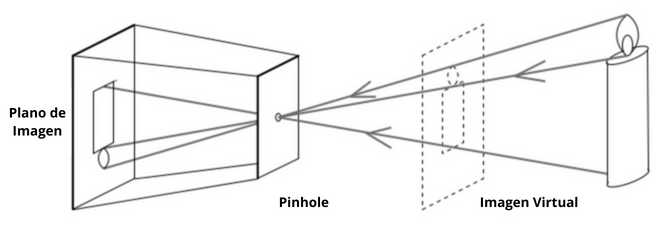
\includegraphics[width=0.6\textwidth]{Figures/Figures_Cap02/pinhole_camera.png}
    \caption{Modelo de cámara \textit{pinhole}.}
    \textit{Nota}. Adaptada de \textit{Computer Vision Group}, 2010 \cite{ComputerVisionGroup}.
    \label{fig:pinhole_camera}
\end{figure}

\subsection{Espacios de Color} \label{sub:espacios_de_color}

La idea de estandarizar el concepto de color surge debido a que los nombres de los colores son insuficientes para toda la gama de combinaciones posibles, otro inconveniente es que un porcentaje de la población solo conoce algunos nombres de colores, y en muchas ocasiones asocian un solo nombre a una gran variedad de un color en específico. 

Se puede entender que los espacios de color o también llamados modelos de color son formas que indican la manera en que un color está definido, permiten aprovechar y analizar toda la información presente dentro de una imagen. Las leyes de Grassman significan que las mezclas de luces de colores se mezclan linealmente, es decir, son una aproximación precisa y lineal\cite{forsyth2011computer}.

Cuando los colores se mezclan linealmente se puede construir un algoritmo sencillo para determinar qué pesos de los primarios se deben de usar para conseguir el color base. Dado que la coincidencia del color es lineal, la combinación de los primarios resulta en una suma ponderada de fuentes de longitud de onda única que es afectada por los pesos específicos de coincidencia. Para cualquier conjunto de primarios (P1, P2, P3) se puede obtener un conjunto de funciones de combinación de colores mediante experimentación\cite{forsyth2011computer}. La Comisión Internacional de la Iluminación CIE (\textit{Commission Internationale d’ eclairage}) ha estandarizado una variedad de sistemas para espacios de color lineales y no lineales.

%Una descripción precisa de colores y estandarizada es un tema de mucha importancia en el sector industrial y tecnológico, pues la mayoría de los fabricantes e investigadores buscan que el mayor porcentaje de los productos tengan el mismo color o al menos sean lo más parecido posible. De esta manera surge la idea de estandarizar el concepto de color, debido a que los nombres de los colores resultan insuficientes para toda la gama de combinaciones posibles, otro inconveniente es que un gran porcentaje de la población conoce solo algunos nombres de colores, y en muchas de las ocasiones asocian un solo nombre a una gran variedad de un color en específico.

%Existe un mecanismo practico y sencillo que permite realizar un emparejamiento de color, tomando como base una combinación de diferentes pesos de los colores primarios hasta empatar el color deseado. Este enfoque también se puede extender para hacer una representación de colores de una superficie si se usa una luz para iluminar la superficie. Este experimento para realizar emparejamiento de colores resulta práctico y en general es el proceso que usan las tiendas de pintura para obtener un color específico con base en combinaciones de pesos de los primarios. Las leyes de Grassman significan que las mezclas de luces de colores se mezclan linealmente, es decir, el emparejamiento es una aproximación precisa y lineal\cite{forsyth2011computer}.

\begin{itemize}
    \item \textbf{Espacios de Color Lineales:}
        \begin{itemize}
            \item \textbf{CIE XYZ:} Creado por la CIE en 1931, las funciones de combinación de color fueron diseñadas para que el resultado obtenido sea positivo en todas partes, es decir, las coordenadas de luz real fueran siempre positivas.
            \item \textbf{RGB:} Es un espacio que utiliza formalmente primarios de una sola onda (R = 645.16nm, G = 526.32nm , B = 444.44nm ). Los colores en este espacio de color se representan mediante un cubo unitario, donde los bordes del cubo son los pesos específicos de las componentes R, G y B.
            \item \textbf{\textit{Opponent Color}:} Es un espacio derivado de RGB que busca tres sistemas de color debido a que existe evidencia acerca de que los primates responden a tres sistemas de color. El más alto responde a la intensidad (Comparaciones claras y obscuras), el segundo compara entre amarillo y azul, el sistema final compara en entre rojo y azul.
\end{itemize}
    \item \textbf{Espacios de Color No Lineales:}
    Un espacio lineal no necesariamente codifica propiedades comunes e importantes en aplicaciones reales. Se excluyen propiedades como tonalidad, saturación y brillo que hacen referencia al cambio de pasar de rojo a verde, de rojo a rosa y de negro a blanco respectivamente. Otra dificultad de los espacios de color lineales es dejar de lado las intuiciones humanas sobre la topología de colores, donde los tonos forman un círculo (Rojo, Naranja, Amarillo, Verde, Cyan, Azul, Morado, Rojo). Esto significa que ninguna coordenada de color en un espacio lineal puede modelar la propiedad de tono\cite{forsyth2011computer}. 

    El espacio HSV( Hue, Saturation, Value), matíz, saturación y valor por sus siglas en inglés es un espacio que basado en RGB y usa una función no lineal para representar las propiedades de tonalidad, saturación y brillo.
    %Por esta razón surge la necesidad de contar con nuevos modelos de color que permitan representar tales propiedades.
\end{itemize}

%En otras palabras, existe una gran cantidad de espacios de color lineales y no lineales que cuentan con características específicas. Sin embargo, la cuestión importante para poder diferenciarlos no es en que sistema de coordenadas se mide el color, sino como se cuenta la diferencia, es decir, la diferencia que existe al momento de buscar reproducir color.

\subsection{Imágenes RGB y su representación en memoria} \label{sub:imágenes_RGB_y_su_representación_en_memoria}
\begin{figure}[h]
    \centering
    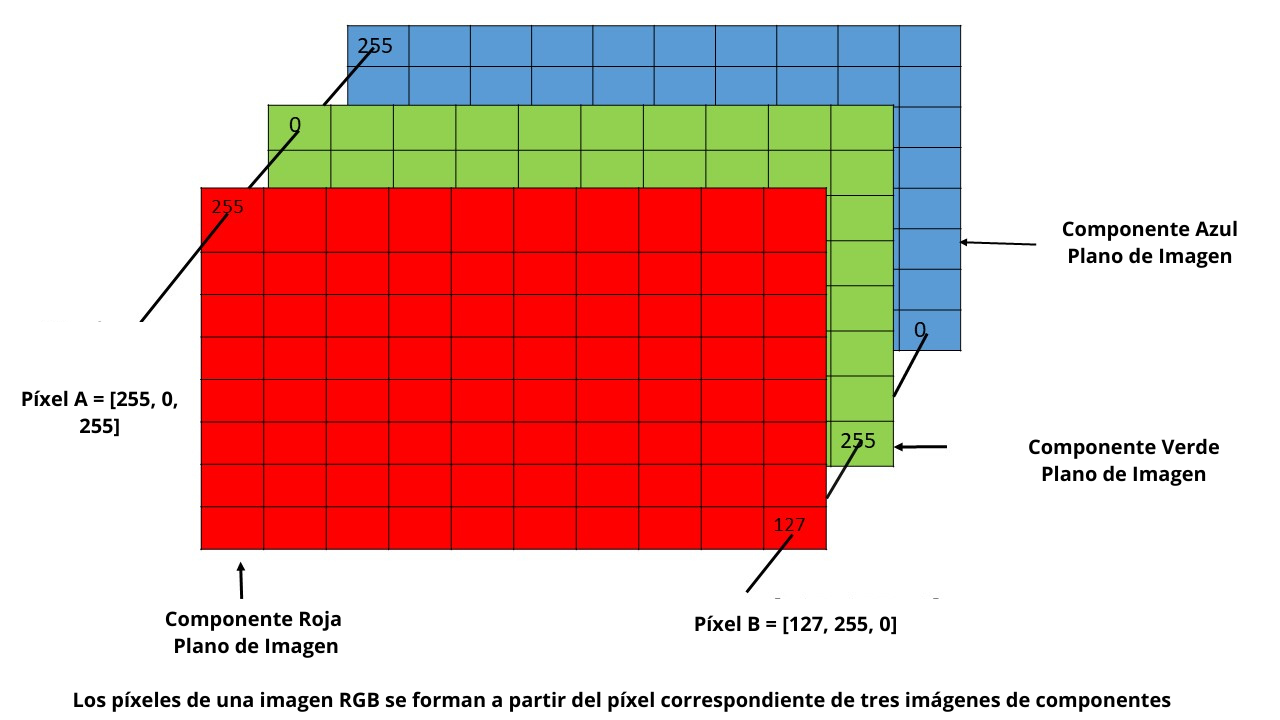
\includegraphics[width=0.75\textwidth]{Figures/Figures_Cap02/rgb_pixels.png}
    \caption{Representación de una Imagen en el espacio RGB.}
    \textit{Nota}. Adaptada de \textit{RGB image representation}, 2018 \cite{RGBImageRepresentation}.
    \label{fig:rgb_pixels}
\end{figure}

Una imagen RGB se puede expresar como tres imágenes diferentes para cada una de las principales componentes RGB (Rojo, Verde, Azul) apiladas una sobre otra, cuando se introducen en un monitor del tipo RGB se combinan para producir una sola imagen de color compuesta. 
La cantidad de píxeles utilizados para representar cada píxel dentro del modelo RGB se denomina profundidad de píxel. Tomando como ejemplo una imagen RGB en la que cada una de las imágenes componentes es de 8-bits en cada píxel (cada píxel es una tripleta de valores [RGB]) tiene una profundidad de píxel de 24 bits, es decir, 3 planos multiplicados por el número de bits (8 bits en este caso), ver \ref{fig:rgb_pixels}. 
% \footnote{\url{https://www.geeksforgeeks.org/matlab-rgb-image-representation/}}

En la práctica, es común escuchar el término de imagen a todo color para referirse a una imagen con profundidad de 24 bits. El número total de colores posibles en una imagen RGB con una profundidad de 24 bits es de $(2^8)^3 = 16 777 216$, es decir, más de 16 millones de combinaciones posibles. De manera que, en cada uno de los ejes (R, G, B) se puede seleccionar un punto en el rango [0, 255], donde el color negro se encuentra en [0, 0, 0] mientras que el blanco se encuentra en [255, 255, 255]\cite{gonzalez2009digital}, la figura \ref{fig:rgb_cube_colors} muestra esto.
% \footnote{\url{https://stackoverflow.com/questions}}
\begin{figure}[h]
    \centering
    
\includegraphics[width=0.3\textwidth]{Figures/Figures_Cap02/rgb_cube_colors.jpg}
    \caption{Cubo de color RGB con profundidad de 24-bits.}
    \textit{Nota}. Tomada de \textit{How to produce RGB cube matrix in python?}, 2014 \cite{stackoverflow}.
    \label{fig:rgb_cube_colors}
\end{figure}

%\textcolor{red}{
%\begin{itemize}
%\item Imágenes RGB y su representación en memoria
%\item Modelo de cámara Pinhole
%\item Espacios de color
%\end{itemize}
%}

\section{Aprendizaje no supervisado} \label{sec:aprendizaje_no_supervisado}

La agrupación de datos en grupos o \textit{clusters} en inglés es una herramienta de la minería de datos con diversos campos de aplicación como biología, seguridad, inteligencia artificial, robótica e incluso búsqueda web. El análisis de grupos es el proceso de distribuir un conjunto de objetos en subconjuntos. Cada subconjunto es conocido como \textit{cluster}, de tal manera que los objetos resultantes dentro de un subconjunto son similares entre sí pero diferentes a los objetos contenidos en otros. Las similitudes y diferencias de los objetos se evalúan en función de las propiedades de los objetos, a menudo, implican medidas de distancia \cite{han2011data}.


\subsection{Agrupamiento (\textit{clustering})}

%El aprendizaje no supervisado es un sinónimo de clustering y se dice que es no supervisado
El agrupamiento es un tipo de aprendizaje no supervisado porque a diferencia del aprendizaje supervisado los datos de entrada no están etiquetados. El agrupamiento es una forma de aprendizaje por observación contrario al aprendizaje mediante ejemplos en el método supervisado. Uno de los retos más grandes del agrupamiento es adaptarse a diferentes tipos y cantidades de datos. Los requerimientos típicos para agrupación en \textit{clusters} dentro de minería de datos son:

\begin{itemize}
    \item \textbf{Escalabilidad:} Necesaria para que algoritmos puedan funcionar de forma aceptable en pequeños y grandes bases de datos.
    
    \item \textbf{Habilidad para tratar con diferentes tipos de atributos:} Muchos algoritmos son diseñados para datos numéricos. Recientemente más y más aplicaciones en el campo de la informática requieren de técnicas de agrupamiento para tipos de datos más complejos como grafos, imágenes y documentos.
    
    \item \textbf{Descubrimiento de \textit{clusters} en forma arbitraria:} Es importante desarrollar algoritmos que puedan detectar \textit{clusters} de forma estándar, diferentes algoritmos determinan \textit{clusters} en base a mediciones de distancia Euclidiana o distancia de Manhattan y centran sus esfuerzos en formar grupos esféricos con tamaño y densidad similares. Sin embargo, un grupo puede tener cualquier forma.
    
    \item \textbf{Habilidad para tratar con datos ruidosos:} Muchos conjuntos de datos reales pueden contener valores atípicos, erróneos o desconocidos. Lecturas de sensores, por ejemplo, a menudo son ruidosas y pueden producir valores incorrectos. Los algoritmos de agrupamiento tienden a ser sensibles al ruido de estas lecturas y pueden generar mala calidad en resultados finales. Por lo tanto, se requiere de métodos robustos ante el ruido. 
    
    \item \textbf{Capacidad para agrupar conjuntos de datos con dimensiones grandes:} Muchos algoritmos de agrupación generan resultados rápidos en conjuntos de datos dimensionalmente pequeños, caso contrarío con lo que sucede con conjuntos más amplíos donde el desempeño de los algoritmos se ve comprometido.
    
    \item \textbf{Interpretabilidad y usabilidad:} Es importante estudiar cual será el campo de aplicación del agrupamiento para realizar una buena elección en el algoritmo a implementar y al final del proceso se obtengan resultados entendibles, usables y con valor para la aplicación.
    
    \item \textbf{Medida de similitud:} Las medidas de similitud juegan un papel importante en el diseño de métodos de agrupamiento. Los métodos basados en distancia a menudo pueden aprovechar técnicas de optimización en el desarrollo, mientras que métodos basados en densidad o continuidad por lo general pueden encontrar grupos con formas arbitrarias.
\end{itemize}

Por lo general, se utiliza el aprendizaje no supervisado para descubrir automáticamente diferentes tipos clases dentro de un conjunto de datos, esta es una clara ventaja del aprendizaje no supervisado frente a otro tipo de aprendizaje porque un \textit{cluster} de objetos puede ser entendido como una clase implícita, pues los elementos de un \textit{cluster} son similares entre si pero diferentes respecto a objetos de otros \textit{clusters} \cite{han2011data}. 

\section{Máquinas de estados finitos} \label{sec:máquinas_de_estados_finitos}

\subsection{Definición} \label{sub:definición}

Las máquinas de estados finitos o FSM (\textit{Finite State Machine}) por sus siglas en inglés son el corazón en la mayoría de los diseños digitales. La idea principal de una FSM es almacenar un conjunto de diferentes estados únicos y realizar transición entre ellos con base en los valores de entrada y el estado actual de la máquina. Una máquina de estados finitos puede ser de dos tipos: Moore y Mealy \cite{wilson2013model}. La primer forma específica que, la salida de la máquina de estados depende puramente de las variables de estado. Por otro lado, en una máquina Mealy la salida puede depender de las variables de estado actuales y valores de entrada a la máquina. El método para describir una FSM es utilizar un diagrama de transición de estados. Este diagrama muestra los estados, salidas y condiciones de transición.

Una alternativa al uso de máquinas de estados finitos es utilizar una técnica llamada Máquina de Estados Algorítmicos (ASM) o carta ASM, esta técnica es útil porque permite separar la ruta de datos y control en un diagrama simple. Una carta ASM es similar a un diagrama de flujo, con acciones y decisiones que pueden ser combinatorias y secuenciales. La diferencia entre FSM Y ASM es la manera gráfica en que se expresan, la forma gráfica de una carta ASM permite definir explícitamente estados, decisiones y resultados, con apariencia similar a un diagrama de flujo. Esto hace que el algoritmo sea más entendible que un diagrama de transición de estados. Una carta ASM tiene tres bloques principales, en \ref{fig:asm_blocks} se ilustran.

\begin{itemize}
    \item \textbf{Estado:} Es representado por una caja rectangular, contiene el valor del estado actual, como un nombre o valor numérico que representa la variable de estado. También puede contener el valor de las salidas según el tipo de máquina de estado (Mealy o Moore).
    \item \textbf{Decisión:}  El bloque de decisión indica diferentes caminos condicionales dependiendo del valor de las variables de entrada. Este bloque es representado en forma de diamante.
    \item \textbf{Salida:} Una salida puede ser condicional o incondicional. Donde; una salida es condicional cuando es precedida por un diamante de decisión (Mealy), por el contrario una salida condicional está presente en un estado sin decisión previa (Moore).
\end{itemize}

\subsection{Formas de implementarlas} \label{sub:formas_de_implementarlas}

Tanto las máquinas de estados finitos (FSM) y las máquinas de estados algorítmicos pueden ser implementadas en diferentes lenguajes de programación, en específico mediante el paradigma de programación imperativa, es decir, la implementación de la máquina debe consistir en una secuencia claramente definida de instrucciones. Las instrucciones se encadenan una detrás de otra para determinar el comportamiento en cada momento y lograr el resultado deseado. Algunos lenguajes que implementan este paradigma son: Python, C, C++, Ensambladores, Ruby, Pascal.
\begin{figure}[h]
    \centering
    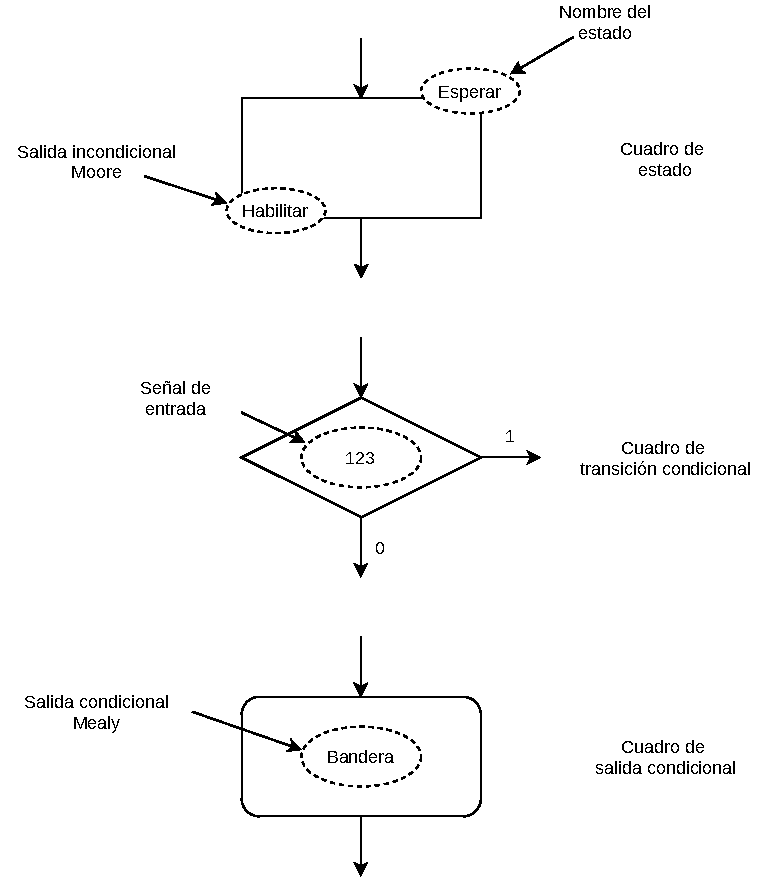
\includegraphics[width=0.5\textwidth]{Figures/Figures_Cap02/asm_chart.pdf}
    \caption{Bloques de una carta ASM.}
    \label{fig:asm_blocks}
\end{figure}


%\textcolor{red}{
%\begin{itemize}
%\item Definición
%\item Formas de implementarlas (memorias y en lenguajes imperativos)
%\end{itemize}
%}

\section{Trabajo relacionado} \label{sec:trabajo_relacionado}

\subsection{Los vehículos Tesla y de Google} \label{sub:los_vehículos_tesla_y_de_google}

\begin{itemize}
    \item \textbf{Tesla:} La compañía Tesla fue fundada en 2003 por un grupo de ingenieros, su objetivo inicial era demostrar que es posible conducir con energía eléctrica y que los vehículos eléctricos pueden ser más rápidos y divertidos de manejar que los vehículos a gasolina. Además, la empresa se enfoca en desarrollar tecnologías que sumen a la conducción autónoma. Tal es el caso de su tecnología Autopilot.
    
    El sistema Autopilot incluye un sofisticado conjunto de cámaras delanteras, traseras, laterales, amplias y estrechas. En adición con una base de red neuronal profunda, el vehículo deconstruye el entorno para incluir mayor nivel de confiabilidad. En la parte de procesamiento, Autopilot añade una capa de hardware con alta velocidad de procesamiento para ejecutar la red neuronal, que es la base de entrenamiento y desarrollo del Autopilot.
    
    Este sistema permite navegar en condiciones viales reales y realizar acciones tediosas durante la conducción como: maniobrar, acelerar y frenar automáticamente dentro del carril. Con su característica Autosteer un Tesla puede navegar en calles estrechas y complejas, con Smart Summon el vehículo puede conducir en entornos y espacios de estacionamiento para efectuar un estacionamiento completamente autónomo. Actualmente las funciones de este sistema requieren una supervisión activa del conductor para no dejar que el vehículo sea completamente autónomo. El uso sin supervisión de un conductor depende de que se logre una confiabilidad superior a las habilidades de conductores humanos, además de demostrarlo con millones de kilómetros recorridos, así como diferentes aprobaciones legales \cite{autopilot}.
    % \footnote{\url{https://www.tesla.com/es_MX/autopilot}}
    
    Tesla no solo produce vehículos totalmente eléctricos y tecnología autónoma, también fabrica productos de almacenamiento y generación de energías limpias que pueden ampliarse de manera ilimitada. 
    % \footnote{\url{https://www.tesla.com/es_MX/about}}
    
    
    
    %En el año 2008 fue lanzado al mercado el Roadster, introdujo tecnología de vanguardia para baterías y sistemas de propulsión eléctrica. Desde entonces Tesla ha desarrollado diferentes modelos de vehículos eléctricos como: el primer sedán 'Model S' \ref{fig:tesla_cars} totalmente eléctrico, años más tarde surgió el 'Model X', como el SUV más rápido, seguro y con mayor capacidad de la historia. Además de vehículos más grandes como camiones y camionetas, el 'Tesla Semi' y 'Cybertruck' respectivamente. \textcolor{red}{Hablar sobre los algoritmos de conducción autónoma y no tanto sobre vehículos eléctricos. }
    
    \item \textbf{Google:}
    Anteriormente conocido como ``Proyecto de vehículo autónomo de Google'' en 2009, Waymo es una empresa de tecnología dedicada a vehículos autónomos, su misión es lograr que pasajeros y objetos lleguen de forma fácil y segura a su destino. Su tecnología busca mejorar el acceso a la movilidad, mientras intenta salvaguardas vidas que se podrían haber perdido en accidentes vehiculares.

    Waymo enfoca sus esfuerzos en el desarrollo de Waymo Driver, su tecnología de conducción autónoma y se divide en dos partes: hardware y software. La parte de hardware incluye un paquete de instrumentación con sistemas lidar, cámaras, radares y una importante plataforma de procesamiento de inteligencia artificial, en conjunto forman una vista de $360^{\circ}$ del ambiente. El software recopila la información de todos los sensores para saber ¿Dónde está?, ¿Qué existe a su alrededor? y ¿Qué debe hacer?. El hardware y software trabaja en conjunto para crear una imagen completa del mundo que rodea al vehículo y navegar de forma segura por las calles \cite{waymo}.
    % \footnote{\url{https://waymo.com/intl/es/faq/}}

    La flota de vehículos de Waymo incluye al Toyota Prius, vehículos deportivos Lexus, un vehículo prototipo (Firefly) y camionetas híbridas Chrysler, ver \ref{fig:waymo_cars}.
\end{itemize}
\begin{figure}[h]
    \centering
    \begin{subfigure}{0.4\textwidth}
         \centering
         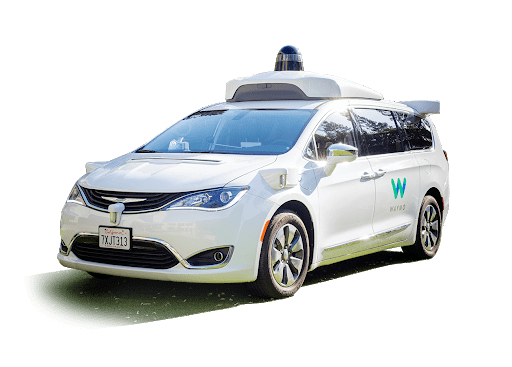
\includegraphics[width=\textwidth]{Figures/Figures_Cap02/waymo_car.png}
         \caption{Vehículo Waymo.}
         \textit{Nota}. Tomada de \textit{Waymo}, 2022 \cite{waymo}.
         \label{fig:waymo_cars}
    \end{subfigure}
    \hfill
    \begin{subfigure}{0.4\textwidth}
         \centering
         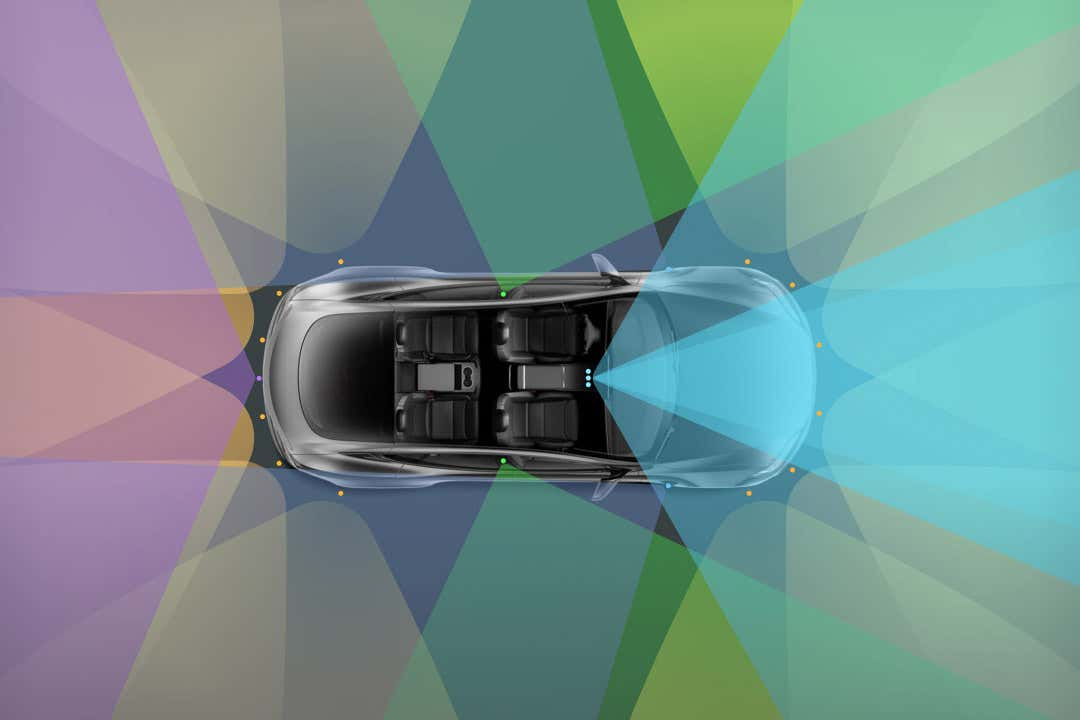
\includegraphics[width=\textwidth]{Figures/Figures_Cap02/tesla_car.jpg}
         \caption{Vehículo Tesla con Autopilot.}
         \textit{Nota}. Tomada de \textit{Autopilot-Tesla}, 2022 \cite{autopilot}.
         \label{fig:tesla_cars}
     \end{subfigure}
    \caption{Vehículos Waymo y Tesla.}
    \label{fig:waymo_tesla_cars}
\end{figure}

\subsection{La categoría AutoModelCar del TMR} \label{sub:la_categoría_autoModelCar_del_TMR}

El Torneo Mexicano de Robótica (TMR) es la competencia de robótica más importante en México. Tiene como principal objetivo motivar e impulsar la investigación y desarrollo de la robótica en busca de un desarrollo integral de nivel internacional. El TMR incluye diferentes categorías de competición con diferentes enfoques \cite{tmr}.
% \footnote{\url{https://www.femexrobotica.org/tmr2022/}}

La categoría AutoModelCar busca incentivar el desarrollo de algoritmos de percepción, planificación y control para vehículos autónomos. Los vehículos no tripulados que participan en esta categoría son modelos a escala 1:10 instrumentados con sensores y actuadores similares a los que tendría un vehículo autónomo en la vida real. Sin embargo, también existe una categoría donde se utilizan simuladores para efectos del vehículo, sensores y actuadores \cite{AutoModelCar}. Esta categoría permite el desarrollo de los mismos algoritmos, además de abrir puertas a la participación a distancia, la figura \ref{fig:tmr_auto_model_car} es una representación de un vehículo a escala utilizado en el TMR en su modalidad presencial. 
% \footnote{\url{https://www.femexrobotica.org/tmr2022/automodelcar/}}
\begin{figure}[h]
    \centering
    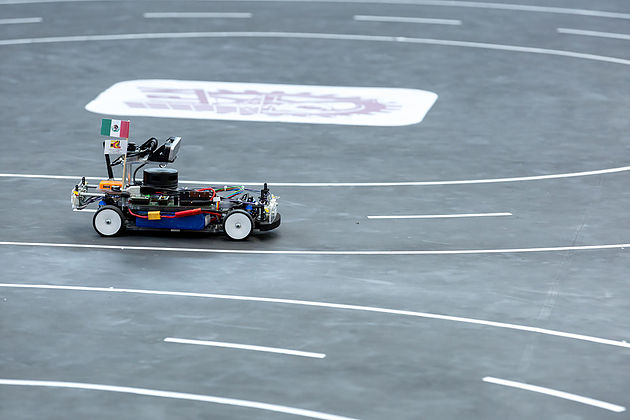
\includegraphics[width=0.5\textwidth]{Figures/Figures_Cap02/automodel_car.jpg}
    \caption{Categoría AutoModelCar del TMR.}
    \textit{Nota}. Tomada de \textit{TMR-AutoModelCar}, 2022 \cite{AutoModelCar}.
    \label{fig:tmr_auto_model_car}
\end{figure}

\subsection{El equipo FUB} \label{sub:el_equipo_FUB}

El trabajo desarrollado por la Universidad Libre de Berlín incluye hardware y software. Cuenta con modelos de vehículos a escala 1:10 y el hardware añade: sensores LIDAR, cámaras RGB con diferentes rangos de visión, puertos USB y adaptadores de red. El software de estos modelos se encuentra sobre la plataforma ROS, este software implementa algoritmos que permiten realizar diferentes tareas de navegación como: detección de líneas de carril, detección de señales de tráfico, control de movimientos, entre otros. Para obtener información más detallada sobre este proyecto visitar \footnote{\url{https://github.com/AutoModelCar/AutoModelCarWiki/wiki}}.






%\textcolor{red}{
%\begin{itemize}
%\item Los vehículos Tesla y de Google
%\item https://github.com/AutoModelCar/AutoModelCarWiki/wiki
%\item La categoría AutoModelCar del TMR
%\item El trabajo hecho en el laboratorio de Biorrobótica
%\end{itemize}
%}

% CONCLUSIONES DEL CAPÍTULO
En este capítulo se presentaron en los conceptos teóricos básicos que serán necesarios a lo largo de este trabajo. Se dio a conocer el término de vehículo autónomo y las características necesarias que requiere para ser considerado como tal, con base en ello se indicó el nivel de autonomía que es pretendido alcanzar al finalizar este proyecto.

En los capítulos siguientes se abordaran de manera específica y detallada muchas de las definiciones aquí mencionadas, también, se expondrán implementaciones de las mismas en aplicaciones para vehículos sin conductor.



